\documentclass[conference]{IEEEtran}
\usepackage[utf8]{inputenc}
\usepackage[T1]{fontenc}
\usepackage[spanish,es-tabla,es-nodecimaldot,es-noshorthands]{babel}
\usepackage{amsmath}
\usepackage{graphicx}
\usepackage{booktabs}
\usepackage{url}
\usepackage{cite}

\renewcommand{\IEEEkeywordsname}{Palabras clave}

\begin{document}

\title{Pronóstico de la vida útil remanente de motores turbofán en C-MAPSS: normalización por condición y ventanas deslizantes con LightGBM}

\author{\IEEEauthorblockN{Carlos Campos Sarabia}
\IEEEauthorblockA{Centro de Investigación Científica y de Educación Superior de Ensenada (CICESE)\\
Introducción a la Ciencia de Datos}}

\maketitle

\begin{abstract}
Predecir cuántos ciclos de vuelo le quedan a un motor antes de fallar (RUL) permite programar su mantenimiento antes de la falla y sin retirarlo antes de tiempo. Se usaron los cuatro subconjuntos de C-MAPSS de NASA (709 motores de entrenamiento y 707 de prueba). Los sensores se normalizaron dentro de cada condición de vuelo, cada ciclo se resumió con ventanas de 10 y 70 ciclos, y todas las decisiones se tomaron con una validación que separa motores completos. El modelo final, LightGBM ajustado con Optuna, obtuvo un RMSE contra el RUL real de 13.10, 21.55, 11.91 y 23.12 ciclos en FD001--FD004 (promedio 17.42), y de 3.5 a 5.8 ciclos cuando al motor le quedan menos de 50. La normalización por condición y las ventanas redujeron el error de validación unas cinco veces más que cambiar de modelo o ajustar sus hiperparámetros. Casi todo el error restante proviene de motores muy sanos, a los que el recorte del objetivo asigna 130 ciclos. La ventaja sobre el mejor notebook público (17.42 contra 17.54) es menor que la incertidumbre de la comparación.
\end{abstract}

\begin{IEEEkeywords}
vida útil remanente, mantenimiento predictivo, C-MAPSS, LightGBM, ventanas deslizantes, validación por grupos.
\end{IEEEkeywords}

\section{Introducción}

Las fallas de motor siguen siendo un riesgo para la aviación comercial. En 1979, el vuelo 191 de American Airlines perdió el motor izquierdo y su pilón al despegar de Chicago por daños introducidos durante un cambio de motor; murieron las 271 personas a bordo y 2 en tierra~\cite{ntsb191}. En 1989, en Kegworth, un álabe del ventilador de un Boeing 737-400 se fracturó por fatiga y la tripulación apagó el motor sano; murieron 47 de las 126 personas a bordo~\cite{aaib92}. En 2010, una grieta por fatiga en un tubo de aceite con un defecto de fabricación causó la falla no contenida de un motor del vuelo 32 de Qantas~\cite{atsb32}, y en 2021 un álabe del ventilador agrietado por fatiga provocó la falla del motor derecho del vuelo 328 de United Airlines~\cite{ntsb328}; en ambos casos la tripulación aterrizó sin víctimas. Tres de los cuatro casos comparten un origen gradual: un daño que crece con los ciclos de operación hasta la falla.

Las fallas también tienen un costo económico. Un avión inmovilizado por mantenimiento no programado (AOG, \emph{aircraft on ground}) cuesta, según estimaciones de Boeing, entre 10\,000 y 20\,000~USD por hora, y hasta 100\,000~USD por hora en algunos casos~\cite{flyingaog}. En 2023, Volaris reportó una pérdida neta de 39 millones de dólares y 200 despidos por problemas con sus motores~\cite{volaris}. El mantenimiento por calendario no resuelve el problema: retira motores sanos antes de tiempo y no anticipa a los que se degradan rápido. Estimar la \emph{vida útil remanente} (RUL) a partir de los sensores permite intervenir según el estado real de cada motor.

C-MAPSS es el conjunto de referencia para este problema~\cite{vollert}. Se plantearon tres preguntas: (P1)~¿un modelo con ventanas deslizantes supera a los notebooks públicos de Kaggle en la prueba oficial de los cuatro subconjuntos?; (P2)~¿qué sensores anticipan de forma consistente la degradación, con coherencia física?; y (P3)~¿tomar en cuenta la condición de operación en el preprocesamiento mejora la predicción en los subconjuntos con varias condiciones?

\section{Datos y métodos}

\subsection{Datos}
C-MAPSS fue generado por NASA Ames con un simulador de un motor turbofán comercial de 90\,000~lbf de empuje~\cite{saxena2008,saxenadata}. Cada motor parte de un desgaste inicial distinto y desconocido; en algún momento aparece una falla que crece hasta la falla del sistema. Cada fila es un ciclo de un motor, con 3 ajustes de operación (altitud, Mach y acelerador) y 21 sensores. Hay cuatro subconjuntos: FD001 (1 condición de vuelo, falla del compresor de alta presión, HPC), FD002 (6 condiciones, HPC), FD003 (1 condición, HPC y ventilador) y FD004 (6 condiciones, HPC y ventilador). En entrenamiento los 709 motores vuelan hasta fallar (160\,359 ciclos, vidas de 128 a 543 ciclos). En prueba, los 707 motores se cortan antes de la falla (entre 19 y 486 ciclos observados) y NASA solo da el RUL real del último ciclo. No hay valores faltantes ni filas duplicadas. Cada motor recibe un identificador único por subconjunto (\texttt{FD002\_15}), porque los números de motor se repiten entre archivos.

\subsection{Objetivo y recorte}
En entrenamiento, $\text{RUL} = \text{último ciclo del motor} - \text{ciclo actual}$. Mientras el motor está sano, sus sensores no cambian: en FD001, el promedio normalizado de Ps30 sube 0.5 desviaciones entre RUL~300 y 130, y casi 3 entre RUL~130 y la falla. Un motor con 300 ciclos por delante y otro con 200 son indistinguibles, y el 42\,\% de los ciclos de entrenamiento está en esa zona. Por eso el objetivo se recorta a 130 ciclos (objetivo lineal por tramos~\cite{heimes}): el modelo aprende a responder ``130 o más'' en la zona sana y concentra su precisión en la de desgaste. La propuesta planteaba recortar a 125; se usó 130 porque ahí está el codo del perfil de los sensores y ningún motor vive menos de 128 ciclos.

\subsection{Sensores y normalización por condición}
Se descartaron los sensores cuya desviación estándar es menor que $10^{-3}$ en alguna condición de vuelo (T2, P2, farB, Nf\_dmd, PCNfR\_dmd y, en FD001 y FD002, epr); quedan 15 o 16 sensores por subconjunto. La condición de cada ciclo se identificó redondeando sus tres ajustes de operación (6 condiciones en FD002 y FD004). En esos subconjuntos la condición mueve los sensores mucho más que el desgaste: T50 marca $\approx$1400~°R a nivel del mar y $\approx$1050~°R a 25\,000 pies. Cada sensor se transformó con un $z$ dentro de su condición,
\begin{equation}
z = \frac{x - \mu_{\text{cond}}}{\sigma_{\text{cond}}},
\end{equation}
con $\mu$ y $\sigma$ calculadas \emph{solo con entrenamiento} y aplicadas igual a prueba. Así, $z$ mide qué tan lejos está cada vuelo de lo normal para su condición, y los saltos entre condiciones desaparecen (Fig.~\ref{fig:norm}).

\begin{figure}[t]
\centering
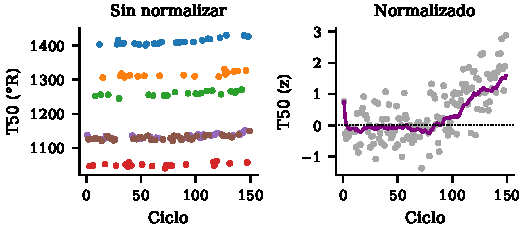
\includegraphics[width=\columnwidth]{figuras/fig_normalizacion.pdf}
\caption{T50 del motor FD002\_1. Izquierda: sin normalizar, cada color es una condición de vuelo y el desgaste queda oculto entre franjas. Derecha: normalizado por condición (gris) y su media móvil de 20 ciclos (morado): el sensor es plano hasta el ciclo $\approx$90 y luego sube hasta $\approx$+2 al fallar.}
\label{fig:norm}
\end{figure}

\subsection{Ventanas deslizantes}
Aun normalizado, un ciclo tiene un ruido de $\approx\pm1$ desviación. Para cada ciclo y cada sensor se resumieron los últimos $w$ ciclos del mismo motor (incluido el actual) en seis estadísticas: valor actual, media, desviación, mínimo, máximo y pendiente de mínimos cuadrados, calculada con promedios móviles como $\text{cov}(t,x)/\text{var}(t)$. La ventana solo mira hacia atrás y, al inicio de la vida, usa los ciclos disponibles. Con $w=70$ resultan 91 columnas en FD001 y FD002 (15 sensores $\times$ 6 + ciclo) y 97 en FD003 y FD004. Una ventana larga es estable pero se atrasa cuando el desgaste se acelera, porque sigue promediando ciclos de cuando el motor estaba sano (Fig.~\ref{fig:ventanas}). Por eso el modelo final combina las estadísticas de $w=10$ y $w=70$ (181 y 193 columnas).

\begin{figure}[t]
\centering
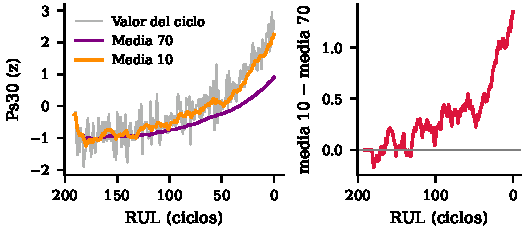
\includegraphics[width=\columnwidth]{figuras/fig_ventanas.pdf}
\caption{Ps30 del motor FD001\_1 contra su RUL. En el último ciclo el sensor vale 2.63 (media centrada de 5 ciclos); la media de 70 ciclos vale 0.90 y la de 10 vale 2.25. Derecha: la diferencia entre ambas medias es $\approx$0 mientras el motor está sano y crece hasta 1.35 al fallar, señal de que el desgaste se acelera.}
\label{fig:ventanas}
\end{figure}

\subsection{Validación por motor y métricas}
La prueba se usó una sola vez para el modelo final. Todas las decisiones se tomaron con \texttt{GroupKFold} de 5 pliegues por motor: cada motor queda completo en entrenamiento o en validación. Los ciclos consecutivos de un motor son casi idénticos. Con un Random Forest, mezclar filas (\texttt{KFold}) estimó un RMSE de 2.52 en FD001, separar motores estimó 10.67, y el error real en un 20\,\% de motores apartados fue 13.74. La validación imita a la prueba: entrena con el RUL recortado, califica contra el RUL real y solo evalúa ciclos cuyo RUL real cae en el rango observado en prueba (7--145, 6--194, 6--145 y 6--195 ciclos en FD001--FD004). Se entrena con uno de cada cinco ciclos, porque los ciclos vecinos aportan casi la misma información. La métrica principal es el RMSE en ciclos. También se reporta el score de NASA~\cite{saxena2008}, que castiga más predecir de más (tarde, $e^{d/10}-1$) que de menos ($e^{-d/13}-1$), con $d$ = predicho $-$ real. La variabilidad se midió repitiendo la validación con 3 semillas, que cambian el reparto de motores en los pliegues, y en P2 con la desviación entre los 20 pliegues.

\subsection{Modelos y ajuste}
Se compararon una línea base que predice el promedio, Ridge, kNN y SVR (con estandarización de columnas), Random Forest, XGBoost~\cite{xgboost} y LightGBM~\cite{lightgbm}, todos con \texttt{scikit-learn}~\cite{sklearn}. LightGBM se agregó a los cinco modelos de la propuesta para compararlo con el notebook \emph{fleet-readiness}~\cite{fleet}, del que se tomó su configuración base (500 árboles, tasa de aprendizaje 0.03, 31 hojas, \texttt{subsample} y \texttt{colsample\_bytree} de 0.8). Sobre el mejor modelo, Optuna~\cite{optuna} con muestreador TPE~\cite{tpe} probó 30 configuraciones, partiendo de la base, y minimizó el RMSE promedio de validación de los cuatro subconjuntos. La mejor (900 árboles, tasa 0.0105, 41 hojas, \texttt{min\_child\_samples} 11, \texttt{subsample} 0.50, \texttt{colsample\_bytree} 0.95, $\lambda$ 0.95) se confirmó con tres semillas antes de entrenar el modelo final con todos los motores de entrenamiento.

Por último, se probó Chronos-2~\cite{chronos2}, un modelo de series de tiempo preentrenado con datos de otros dominios, usado congelado como extractor de características. Recibe los últimos 64 ciclos de los sensores normalizados y devuelve un resumen (\emph{embedding}) de 1\,054 a 1\,056 valores: dos vectores de 512 promediados entre sensores, más la media y la desviación de cada sensor. Dentro de cada pliegue, ese resumen se redujo a 32 componentes con PCA y se agregó a las columnas de las ventanas. Para replicar el trabajo, el código, los resultados intermedios y las predicciones están en el repositorio\footnote{\url{https://github.com/Elsarabia15/ICD-2026}, carpeta \texttt{Proyecto} (notebook \texttt{Proyecto-CMAPSS-v2.ipynb}).}.

\section{Resultados}

\begin{table}[t]
\centering
\caption{RMSE de validación (Random Forest) según la longitud de la ventana: promedio de 3 semillas y ruido entre semillas.}
\label{tab:ventanas}
\footnotesize
\setlength{\tabcolsep}{4pt}
\begin{tabular}{@{}rrrrrrr@{}}
\toprule
Ventana & FD001 & FD002 & FD003 & FD004 & Prom. & $\pm$ \\
\midrule
1   & 20.60 & 29.95 & 20.48 & 31.74 & 25.69 & 0.09 \\
10  & 20.15 & 29.38 & 19.88 & 31.34 & 25.19 & 0.09 \\
30  & 16.64 & 28.03 & 15.68 & 29.44 & 22.45 & 0.07 \\
50  & 14.29 & 26.28 & 14.33 & 28.02 & 20.73 & 0.05 \\
\textbf{70} & 13.55 & 25.37 & 14.18 & 27.52 & \textbf{20.16} & 0.01 \\
100 & 13.56 & 25.03 & 14.45 & 27.34 & 20.10 & 0.04 \\
\bottomrule
\end{tabular}
\end{table}

\textbf{Ventanas.} El error baja de 25.69 sin ventana a 20.16 con 70 ciclos y se estabiliza de 70 a 100 (Tabla~\ref{tab:ventanas}). Se eligió la ventana más corta a menos de 1\,\% del mejor promedio (70), porque deja menos motores de prueba con la ventana incompleta: en FD002, 50 motores tienen menos de 70 ciclos y 91 menos de 100. El ruido entre semillas ($\le$0.09) es mucho menor que las diferencias entre ventanas cortas y largas.

\begin{table}[t]
\centering
\caption{RMSE de validación por modelo y por mejora sucesiva. Las filas con $\pm$ usan 3 semillas; las demás, una sola. $^{*}$Evaluado solo en uno de cada cinco ciclos.}
\label{tab:modelos}
\footnotesize
\setlength{\tabcolsep}{3pt}
\begin{tabular}{@{}lrrrrrr@{}}
\toprule
Modelo & FD001 & FD002 & FD003 & FD004 & Prom. & $\pm$ \\
\midrule
Promedio & 41.95 & 52.87 & 44.97 & 53.65 & 48.36 & \\
Ridge & 20.48 & 31.03 & 19.98 & 33.36 & 26.22 & \\
kNN & 19.41 & 31.72 & 19.01 & 32.31 & 25.61 & \\
SVR & 14.74 & 27.06 & 14.92 & 28.08 & 21.20 & \\
Random Forest & 13.69 & 25.34 & 14.05 & 27.51 & 20.15 & \\
XGBoost & 13.66 & 24.62 & 13.24 & 26.80 & 19.58 & \\
LightGBM & 12.82 & 24.49 & 12.77 & 26.61 & 19.17 & \\
\midrule
+ ventanas 10\,+\,70 & 12.50 & 24.24 & 12.61 & 26.43 & 18.95 & \\
\quad base, 3 semillas & 12.31 & 24.25 & 12.72 & 26.48 & 18.94 & 0.01 \\
+ Optuna & 12.17 & 24.05 & 12.56 & 26.34 & 18.78 & 0.01 \\
\midrule
LightGBM$^{*}$ & 12.18 & 23.91 & 12.53 & 26.30 & 18.73 & 0.01 \\
+ Chronos-2$^{*}$ & 12.12 & 23.86 & 12.17 & 26.02 & 18.54 & 0.08 \\
\bottomrule
\end{tabular}
\end{table}

\textbf{Modelos y ajuste.} Todos los modelos superan con amplitud a la línea base (Tabla~\ref{tab:modelos}). Los de árboles son los mejores y LightGBM tiene el menor error en los cuatro subconjuntos. Agregar la ventana de 10 ciclos mejora los cuatro (19.17 $\rightarrow$ 18.95), mientras que 30\,+\,70 mejora menos (19.11). Optuna baja el error de 18.94 a 18.78 con las tres semillas, una diferencia 16 veces mayor que el ruido. En las columnas del modelo final, la media de 10 ciclos concentra el 59\,\% de la ganancia, la pendiente de 70 ciclos el 19\,\% y el valor de un solo ciclo el 0.4\,\%.

\textbf{Condición de operación (P3).} Con el mismo LightGBM, normalizar con una sola media por sensor da un RMSE de validación de 30.54~$\pm$~0.02 en FD002 y FD004. Agregar la condición como columna da el mismo valor (30.54~$\pm$~0.01). Normalizar dentro de cada condición lo baja a 25.20~$\pm$~0.05; en prueba, el error pasa de 26.96 a 22.34.

\begin{table}[t]
\centering
\caption{Prueba oficial: RMSE contra el RUL real, contra el RUL recortado a 125 y por zona de RUL real (entre paréntesis, motores en la zona).}
\label{tab:test}
\footnotesize
\setlength{\tabcolsep}{2.6pt}
\begin{tabular}{@{}lrrrrrr@{}}
\toprule
 & Real & $\le$125 & $<$50 & 50--130 & $>$130 & Tarde \\
\midrule
FD001 & 13.10 & 12.28 & 3.5 (30) & 15.1 (62) & 18.4 (8) & 54\,\% \\
FD002 & 21.55 & 10.36 & 4.9 (87) & 14.3 (117) & 41.4 (55) & 42\,\% \\
FD003 & 11.91 & 11.01 & 4.1 (29) & 13.9 (60) & 14.0 (11) & 47\,\% \\
FD004 & 23.12 & 12.56 & 5.8 (79) & 17.3 (109) & 40.2 (60) & 46\,\% \\
\midrule
Prom. & 17.42 & 11.55 & & & & 47\,\% \\
\bottomrule
\end{tabular}
\end{table}

\begin{figure}[t]
\centering
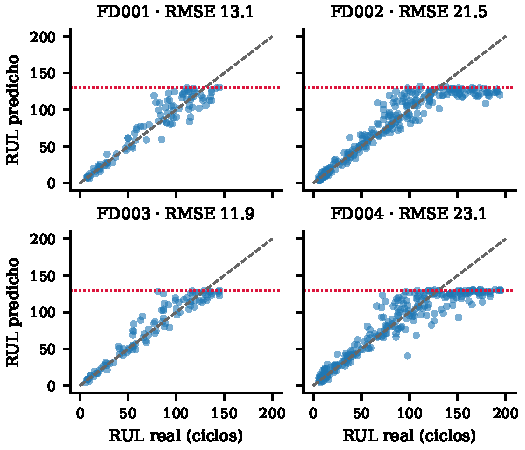
\includegraphics[width=\columnwidth]{figuras/fig_dispersion.pdf}
\caption{RUL predicho contra real en el último ciclo de los 707 motores de prueba. Cerca de la falla los puntos siguen la diagonal; los motores con más de 130 ciclos restantes forman una meseta en $\approx$130 (línea roja), por el recorte.}
\label{fig:disp}
\end{figure}

\textbf{Prueba.} El RMSE contra el RUL real es de 17.42 en promedio (Tabla~\ref{tab:test}). Cerca de la falla (RUL $<$ 50) es de 3.5 a 5.8 ciclos, con un sesgo de $+$0.2 a $+$2.4 ciclos. Entre 50 y 130 sube a 14--17 ciclos. En los motores con más de 130 ciclos restantes alcanza 40 ciclos en FD002 y FD004, siempre por defecto (sesgo de $-$13 a $-$37; Fig.~\ref{fig:disp}). El 47\,\% de las predicciones son tardías. La suma del score de NASA es de 290, 3\,003, 320 y 2\,797 en FD001--FD004.

\begin{table}[t]
\centering
\caption{RMSE de prueba contra el RUL real frente a trabajos públicos (protocolo oficial, una predicción por motor).}
\label{tab:kaggle}
\footnotesize
\setlength{\tabcolsep}{2.6pt}
\begin{tabular}{@{}lrrrrr@{}}
\toprule
 & FD001 & FD002 & FD003 & FD004 & Prom. \\
\midrule
Random Forest, 1 ciclo~\cite{kirstein} & 17.96 & --- & --- & --- & --- \\
LSTM, 30 ciclos~\cite{momt} & 15.30 & --- & --- & --- & --- \\
GRU + atención~\cite{rulcodes} & 14.21 & 27.99 & 14.64 & 26.78 & 20.91 \\
Chronos-2 + LightGBM~\cite{fleet} & \textbf{11.79} & 23.38 & \textbf{11.13} & 23.86 & 17.54 \\
\midrule
LightGBM 10\,+\,70 (este trabajo) & 13.10 & 21.55 & 11.91 & 23.12 & 17.42 \\
\quad + Chronos-2 & 12.66 & \textbf{21.51} & 11.90 & \textbf{22.79} & \textbf{17.22} \\
\bottomrule
\end{tabular}
\end{table}

\textbf{Comparación (P1).} De siete notebooks de Kaggle revisados, solo tres reportan el protocolo oficial (Tabla~\ref{tab:kaggle}). Este trabajo supera a los dos que solo reportan FD001 y tiene el menor promedio, pero \emph{fleet-readiness} es mejor en FD001 y FD003. Con Chronos-2, el RMSE de prueba baja de 17.42 a 17.22. Contra el RUL recortado a 125, \emph{fleet-readiness} obtiene 10.59 y este trabajo 11.35.

\begin{figure}[t]
\centering
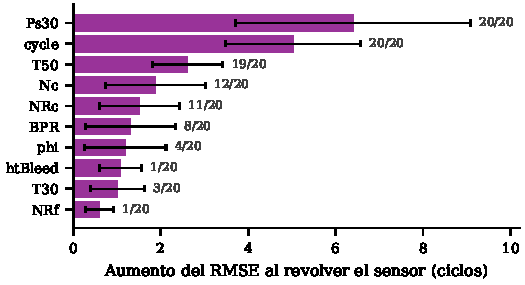
\includegraphics[width=\columnwidth]{figuras/fig_permutacion.pdf}
\caption{Importancia por permutación (P2): aumento medio del RMSE de validación al revolver las 12 columnas de un sensor, con su desviación entre los 20 pliegues (5 por subconjunto). A la derecha, en cuántos pliegues quedó entre los 5 más importantes.}
\label{fig:perm}
\end{figure}

\textbf{Sensores (P2).} Ps30 está entre los cinco más importantes en los 20 pliegues ($+$6.4 ciclos de RMSE al revolverlo), T50 en 19 ($+$2.6), y Nc y NRc en 12 y 11 (Fig.~\ref{fig:perm}). P15, epr, W31 y W32 aportan menos de 0.3 ciclos.

\section{Discusión}

\textbf{Los datos pesaron más que el modelo.} Normalizar por condición ($-$5.3 ciclos en FD002 y FD004) y usar ventanas ($-$5.5) redujeron el error mucho más que cambiar de Random Forest a LightGBM ($-$1.0), agregar la ventana corta ($-$0.2), ajustar con Optuna ($-$0.16) o agregar Chronos-2 ($-$0.19). El experimento de P3 muestra por qué. La condición como columna no ayuda, porque la ventana de 70 ciclos ya mezcló vuelos de seis condiciones y una columna con la condición del ciclo actual no puede deshacer esa mezcla. La normalización corrige cada vuelo \emph{antes} de promediar, así que la ventana solo ve el desgaste. Un modelo más complejo no recupera información que el preprocesamiento borró.

\textbf{Las dos ventanas aportan cosas distintas.} El modelo toma el nivel de la ventana corta y la tendencia de la larga, y casi ignora el valor de un solo ciclo. La Fig.~\ref{fig:ventanas} muestra el mecanismo: cerca de la falla, la media de 70 ciclos se atrasa 1.73 desviaciones y la de 10 solo 0.38. Esa diferencia, que crece cuando el desgaste se acelera, no la da ninguna ventana por sí sola.

\textbf{Un RMSE de 17.42 no describe un solo comportamiento.} El error depende de qué tan lejos está el motor de fallar. Cerca de la falla, donde se decide sacar un motor de servicio, el modelo se equivoca unos 5 ciclos y sin tendencia a avisar tarde. El error grande está en los motores muy sanos y es una consecuencia buscada del recorte: a un motor con 190 ciclos restantes se le predice $\approx$130, un error del lado seguro que no cambia la decisión de mantenimiento. FD002 y FD004 tienen más error total porque tienen 55 y 60 motores sanos en prueba, contra 8 y 11 en FD001 y FD003, y no porque el modelo funcione peor en ellos: contra el RUL recortado a 125, los cuatro quedan entre 10.4 y 12.6. La validación fue una buena guía, con 18.78 en validación y 17.42 en prueba. En FD002 y FD004 la prueba sale mejor porque el rango de validación incluye proporcionalmente más ciclos sanos que los motores de prueba.

\textbf{Los sensores elegidos tienen sentido físico, pero la importancia no es causalidad.} Los cuatro subconjuntos incluyen degradación del HPC. Un compresor gastado cambia la presión estática a su salida (Ps30), exige más combustible para el mismo empuje y eleva la temperatura de salida de la turbina de baja presión (T50); la velocidad del núcleo (Nc) se ajusta para compensar. Que Ps30 y T50 salgan arriba con la ganancia y con la permutación hace robusta esa conclusión. En cambio, T30 y htBleed tienen mucha ganancia y poca importancia por permutación: las temperaturas suben juntas y el modelo puede reemplazar una por otra. No se puede concluir que T30 sea irrelevante, solo que es redundante para este modelo.

\textbf{Qué no se puede concluir de la comparación.} El menor promedio frente a \emph{fleet-readiness} (17.42 contra 17.54) no prueba un modelo mejor. Las diferencias por subconjunto (0.7 a 1.8 ciclos) son del mismo orden que los intervalos de confianza de $\approx\pm$2 ciclos que ese trabajo reporta con 100 motores de prueba, y los dos trabajos optimizan métricas distintas: ellos recortan a 125 y califican contra el RUL recortado. Este trabajo gana en FD002 y FD004, que tienen muchos motores sanos y donde el recorte a 130 queda más cerca del RUL real. Pierde en FD001 y FD003, donde la diferencia está en la zona de desgaste. Una explicación posible, no probada aquí, es que ellos agregan la deriva de cada sensor respecto a los primeros ciclos del propio motor. Chronos-2 mejora la validación más allá del ruido, pero solo 0.2 ciclos, a cambio de una GPU y un modelo de 28 millones de parámetros. Las ventanas 10\,+\,70 ya capturan casi todo lo que aporta.

\textbf{Respuestas.} P1: en parte; el modelo supera a los notebooks públicos en promedio y en FD002 y FD004, pero no en los cuatro subconjuntos. P2: sí; Ps30 y T50, seguidos de Nc y NRc, de forma consistente y coherente con la degradación del HPC. P3: sí; normalizar por condición reduce el error 5.3 ciclos en validación y 4.6 en prueba.

\section{Limitaciones}

\begin{itemize}
\item \textbf{Datos simulados.} C-MAPSS modela la pérdida de eficiencia y de flujo de módulos del motor, no grietas, defectos de fabricación ni errores de montaje como los de los casos de la introducción. El modelo no se ha validado con motores reales.
\item \textbf{Incertidumbre subestimada.} Las semillas solo reparten de otra forma los mismos motores, por lo que su ruido ($\le$0.09) subestima la variabilidad real. En prueba no se calcularon intervalos de confianza, y el modelo da una predicción puntual sin incertidumbre~\cite{vollert,rostami}.
\item \textbf{Decisiones no validadas.} El recorte a 130 se eligió con el perfil de los sensores y la literatura, no con validación. El rango de evaluación de la validación usa el RUL mínimo y máximo de prueba (no el de cada motor).
\item \textbf{Uso de la prueba.} La prueba se usó para el modelo final y, de nuevo, para el experimento con Chronos-2.
\item \textbf{Historias cortas.} Con pocos ciclos observados, la ventana está incompleta y un motor de vida corta no se distingue de uno de vida larga: el motor FD001\_1 de prueba, con 31 ciclos, se predijo en 127.5 cuando le quedaban 112.
\end{itemize}

\section{Conclusiones}

Un LightGBM con normalización por condición y ventanas de 10 y 70 ciclos predice el RUL de C-MAPSS con 17.42 ciclos de error promedio y unos 5 ciclos cerca de la falla, al nivel del mejor notebook público. El hallazgo principal es que el preprocesamiento, más que el modelo, determinó el desempeño: quitar el efecto de la condición de vuelo y resumir la historia reciente de cada sensor explican casi toda la mejora. El trabajo futuro debe elegir el recorte con validación, estimar intervalos de confianza por motor, agregar la deriva respecto a la línea base de cada motor y probar el método con datos de operación reales.

\section*{Declaración de uso de IA generativa}
En este trabajo se usó Claude Opus 5.5 (Anthropic) como apoyo en la escritura y el formato: redactar el texto a partir de un borrador y una estructura del autor, darle formato en LaTeX y generar las figuras a partir de los resultados del notebook. El análisis, los experimentos y las decisiones del proyecto son del autor, quien revisó el contenido final y es responsable de él.

\begin{thebibliography}{99}
\footnotesize

\bibitem{ntsb191} National Transportation Safety Board, ``Aircraft accident report: American Airlines, Inc., DC-10-10, N110AA, Chicago-O'Hare International Airport, Chicago, Illinois, May 25, 1979,'' NTSB-AAR-79-17, Washington, DC, 1979.

\bibitem{aaib92} Air Accidents Investigation Branch, ``Report on the accident to Boeing 737-400, G-OBME, near Kegworth, Leicestershire on 8 January 1989,'' Aircraft Accident Report 4/1990, Londres, 1990.

\bibitem{atsb32} Australian Transport Safety Bureau, ``In-flight uncontained engine failure, Airbus A380-842, VH-OQA, overhead Batam Island, Indonesia, 4 November 2010,'' AO-2010-089, 2013.

\bibitem{ntsb328} National Transportation Safety Board, ``United Airlines flight 328, Boeing 777-222, N772UA, engine failure, Broomfield, Colorado, February 20, 2021,'' investigación DCA21FA085, 2023. [En línea]. Disponible: \url{https://www.ntsb.gov/investigations/Pages/DCA21FA085.aspx}

\bibitem{flyingaog} Flying Magazine, ``AOG: When an airplane can't fly.'' [En línea]. Disponible: \url{https://www.flyingmag.com/aog-when-an-airplane-or-we-cant-fly}

\bibitem{volaris} A. Munguía, ``Volaris despide a 200 empleados por problemas con motores,'' \emph{El Financiero}, 31 oct. 2023.

\bibitem{vollert} S. Vollert y A. Theissler, ``Challenges of machine learning-based RUL prognosis: A review on NASA's C-MAPSS data set,'' en \emph{Proc. 26th IEEE Int. Conf. Emerging Technologies and Factory Automation (ETFA)}, 2021.

\bibitem{saxena2008} A. Saxena, K. Goebel, D. Simon y N. Eklund, ``Damage propagation modeling for aircraft engine run-to-failure simulation,'' en \emph{Proc. Int. Conf. Prognostics and Health Management (PHM08)}, Denver, CO, 2008.

\bibitem{saxenadata} A. Saxena y K. Goebel, ``Turbofan engine degradation simulation data set,'' NASA Prognostics Data Repository, NASA Ames Research Center, Moffett Field, CA, 2008.

\bibitem{heimes} F. O. Heimes, ``Recurrent neural networks for remaining useful life estimation,'' en \emph{Proc. Int. Conf. Prognostics and Health Management (PHM08)}, Denver, CO, 2008.

\bibitem{xgboost} T. Chen y C. Guestrin, ``XGBoost: A scalable tree boosting system,'' en \emph{Proc. 22nd ACM SIGKDD Int. Conf. Knowledge Discovery and Data Mining}, 2016, pp. 785--794.

\bibitem{lightgbm} G. Ke \emph{et al.}, ``LightGBM: A highly efficient gradient boosting decision tree,'' en \emph{Advances in Neural Information Processing Systems 30}, 2017.

\bibitem{sklearn} F. Pedregosa \emph{et al.}, ``Scikit-learn: Machine learning in Python,'' \emph{J. Mach. Learn. Res.}, vol. 12, pp. 2825--2830, 2011.

\bibitem{fleet} A. E. Elsamahy, ``Fleet readiness: Engine RUL on NASA C-MAPSS,'' notebook de Kaggle, 2026. [En línea]. Disponible: \url{https://www.kaggle.com/code/amiresamelsamahy/fleet-readiness-engine-rul-on-nasa-c-mapss}

\bibitem{optuna} T. Akiba, S. Sano, T. Yanase, T. Ohta y M. Koyama, ``Optuna: A next-generation hyperparameter optimization framework,'' en \emph{Proc. 25th ACM SIGKDD Int. Conf. Knowledge Discovery and Data Mining}, 2019, pp. 2623--2631.

\bibitem{tpe} J. Bergstra, R. Bardenet, Y. Bengio y B. Kégl, ``Algorithms for hyper-parameter optimization,'' en \emph{Advances in Neural Information Processing Systems 24}, 2011.

\bibitem{chronos2} A. F. Ansari \emph{et al.}, ``Chronos-2: From univariate to universal forecasting,'' preimpresión, Amazon Web Services, 2025. Modelo: \url{https://huggingface.co/autogluon/chronos-2-small}

\bibitem{kirstein} C. Kirstein, ``Predictive maintenance NASA turbofan regression,'' notebook de Kaggle, 2022. [En línea]. Disponible: \url{https://www.kaggle.com/code/carlkirstein/predictive-maintenance-nasa-turbofan-regression}

\bibitem{momt} Y. Momt, ``RUL prediction using LSTM for aircraft engine,'' notebook de Kaggle, 2023. [En línea]. Disponible: \url{https://www.kaggle.com/code/yahyamomtaz/rul-prediction-using-lstm-for-aircraft-engine}

\bibitem{rulcodes} B. Sahoo, ``rul\_codes\_open: Remaining useful life prediction codes,'' repositorio de GitHub. [En línea]. Disponible: \url{https://github.com/biswajitsahoo1111/rul_codes_open}

\bibitem{rostami} A. S. Sadati Rostami y S. Harifi, ``Phase-aware probabilistic multitask learning for reliable RUL prediction in turbofan engines,'' \emph{IEEE Access}, 2026, doi: 10.1109/ACCESS.2026.3744269.

\end{thebibliography}

\end{document}
